% ******************************************************** %
%              TEMPLATE DE INFORME ORGA2 v0.1              %
% ******************************************************** %
% ******************************************************** %
%                                                          %
% ALGUNOS PAQUETES REQUERIDOS (EN UBUNTU):                 %
% ========================================
%                                                          %
% texlive-latex-base                                       %
% texlive-latex-recommended                                %
% texlive-fonts-recommended                                %
% texlive-latex-extra?                                     %
% texlive-lang-spanish (en ubuntu 13.10)                   %
% ******************************************************** %


\documentclass[a4paper]{article}
\usepackage[spanish]{babel}
\usepackage[utf8]{inputenc}
\usepackage{charter}   % tipografia
\usepackage{graphicx}
%\usepackage{makeidx}
\usepackage{paralist} %itemize inline
\usepackage{subcaption}


%\usepackage{float}
%\usepackage{amsmath, amsthm, amssymb}
%\usepackage{amsfonts}
%\usepackage{sectsty}
%\usepackage{charter}
%\usepackage{wrapfig}
%\usepackage{listings}
%\lstset{language=C}

% \setcounter{secnumdepth}{2}
\usepackage{underscore}
\usepackage{caratula}
\usepackage{url}
\usepackage{ragged2e}
\usepackage{hyperref}
\usepackage{pdfpages}


% ********************************************************* %
% ~~~~~~~~              Code snippets             ~~~~~~~~~ %
% ********************************************************* %

\usepackage{color} % para snipets de codigo coloreados
\usepackage{fancybox}  % para el sbox de los snipets de codigo

\definecolor{litegrey}{gray}{0.94}

\newenvironment{codesnippet}{%
	\begin{Sbox}\begin{minipage}{\textwidth}\sffamily\small}%
	{\end{minipage}\end{Sbox}%
		\begin{center}%
		\vspace{-0.4cm}\colorbox{litegrey}{\TheSbox}\end{center}\vspace{0.3cm}}



% ********************************************************* %
% ~~~~~~~~         Formato de las páginas         ~~~~~~~~~ %
% ********************************************************* %

\usepackage{fancyhdr}
\pagestyle{fancy}

%\renewcommand{\chaptermark}[1]{\markboth{#1}{}}
\renewcommand{\sectionmark}[1]{\markright{\thesection\ - #1}}

\fancyhf{}

\fancyhead[LO]{Sección \rightmark} % \thesection\ 
\fancyfoot[LO]{\small{Ivo Pajor, Laureano Muñiz, Luciana Gorosito}}
\fancyfoot[RO]{\thepage}
\renewcommand{\headrulewidth}{0.5pt}
\renewcommand{\footrulewidth}{0.5pt}
\setlength{\hoffset}{-0.8in}
\setlength{\textwidth}{16cm}
%\setlength{\hoffset}{-1.1cm}
%\setlength{\textwidth}{16cm}
\setlength{\headsep}{0.5cm}
\setlength{\textheight}{25cm}
\setlength{\voffset}{-0.7in}
\setlength{\headwidth}{\textwidth}
\setlength{\headheight}{13.1pt}

\renewcommand{\baselinestretch}{1.1}  % line spacing

% ******************************************************** %


\begin{document}


\thispagestyle{empty}
\materia{Organización del Computador II}
\submateria{Segundo Cuatrimestre de 2020}
\titulo{Trabajo Práctico III}
\subtitulo{System Programming}
\integrante{Ivo Pajor}{460/19}{ivo_pajor@hotmail.com}
\integrante{Laureano Muñiz}{498/19}{lau2000m@hotmail.com}
\integrante{Luciana Gorosito}{577/18}{lugorosito0@gmail.com}

\maketitle


\thispagestyle{empty}
\vfill


\thispagestyle{empty}
\vspace{3cm}
\tableofcontents
\newpage


%\normalsize
\newpage

\section{Introducción}
\justify
El objetivo de este trabajo práctico es aplicar gradualmente los conceptos de \textit{System Programming} vistos en las clases teóricas y prácticas, mediante la implementación de una serie de ejercicios que, inspirados en la serie \textit{Rick y Morty}, en conjunto conformarán un kernel o un pequeño sistema operativo. 



\section{Desarrrollo}
\justify
A continuación detallamos las implementaciones de los ejercicios del trabajo práctico.

\subsection{Ejercicio 1}
\justify
Para la realización de este ejercicio analizamos las estructuras \textbf{gdt_entry_t} y \textbf{gdt_descriptor_t} definidas por la cátedra. En esta implementación, la Tabla de Descriptores Globales(GDT) es un arreglo de  \textbf{gdt_entry_t} y su descriptor, que luego cargaremos en GDTR, es del tipo \textbf{gdt_descriptor_t}.\par
\justify
Siguiendo lo indicado en el primer item, definimos a partir del índice 10, 4 descriptores de segmento en la GDT utilizando la estructura \textbf{gdt_entry_t}, atendiendo a las propiedades particulares de cada segmento. Así definimos las entradas de dos segmentos de código de nivel
0 y 3 y de dos segmentos de datos, también de nivel 0 y 3. Puesto que estos segmentos deben direccionar los primeros 201 MB de memoria establecimos en todos el bit de G en 1, y definimos su base en 0x00000000 y su limite en 0x00C8FF. Además, como son segmentos de código o datos de 32 bits, los bit S y D/B se encuentran seteados en 1 y el bit L en 0. Los bits de DPL de cada uno están seteados en 0 o en 3 de acuerdo con el nivel de privilegio que le corresponda. Por último, los bits de tipo están seteados como 0xA en caso de tratarse de un segmento de código y como 0x2 en caso de tratarse de un segmento de datos. En todos, el bit P se setea en 1 para reflejar que los segmentos están presentes. En el caso del bit de AVL, como es un bit reservado lo seteamos en 0.

\begin{figure}[h]
	\centering
	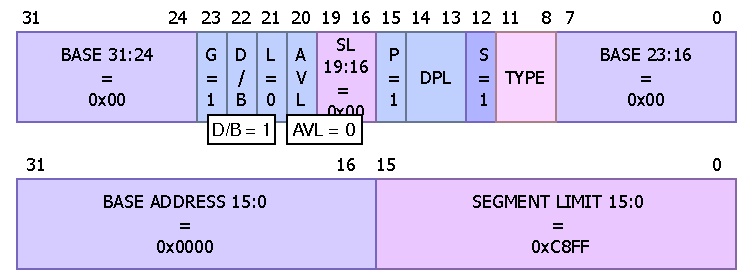
\includegraphics[scale=0.8]{img/GDTdescriptor.pdf}
	\caption{Esquema general de un descriptor de la GDT para los 4 segmentos.}
\end{figure}


\justify
Realizando lo pedido en el item b, pasamos a modo protegido. Para poder hacer esto modificamos el archivo kernel.asm, allí deshablitamos las interrupciones, cargamos en el registro GDTR la estructura \textbf{gdt_descriptor_t} y modificamos el ultimo bit del registro de control CR0, es decir, seteamos en 1 el bit de \textit{Protection Enable}. Posteriormente, escribimos el código necesario para saltar efectivamente a modo protegido. Debido a que este salto se consigue haciendo un \textit{far jump} a la próxima instrucción, designamos una etiqueta llamada \textbf{modo_protegido} a partir de la cual obtendremos el offset, mientras que como selector utilizamos el correspondiente al segmento de código de nivel 0. Además, seteamos la pila del kernel en la dirección 0x25000, es decir, en la base de la pila. Una vez que pasamos a modo protegido, cargamos correctamente los selectores de segmento, en los registros ds, es, fs, gs, ss, usando como registro auxiliar ax, donde se encontraba el selector de segmento de nivel 0 (RPL = 0).


\justify
Seguidamente, definimos otra entrada en la GDT destinada a un segmento de vídeo de nivel 0 (DPL = 0). A diferencia de los cuatro segmentos anteriores, la base de este segmento es distinta de 0, por lo que los campos de la base fueron ser completados con el valor 0x000B8000. Como la pantalla es de 80x50 y como cada pixel ocupa 2 bytes, el límite de este segmento es 0x01F3F. Como este límite entra en 20 bits, el bit de granularidad de este descriptor queda en 0. Además, al ser un segmento de datos de lectura y escritura el tipo es 0x02 y el bit de s queda seteado en 1. Como en las entradas anteriores, los bits de AVL y L quedan en 0, mientras que los bits de present y D/B quedan en 1.  

\begin{figure}[h]
	\centering
	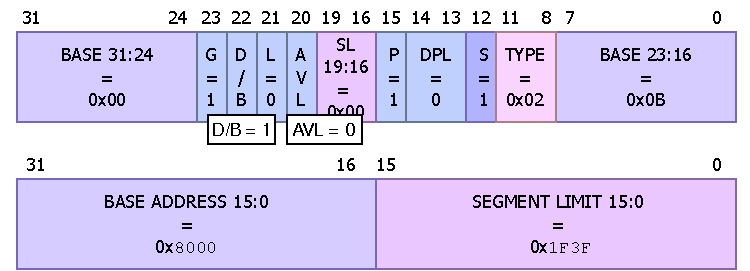
\includegraphics[scale=0.8]{img/DescriptorVideo.pdf}
	\caption{Esquema del descriptor de segmento de video.}
\end{figure}

\justify
Para finalizar este ejercicio, realizamos un rutina encargada de limpiar la pantalla, y pintar el área del mapa de color verde, junto con las barras de los jugadores Rick y Morty. Inicialmente, esta rutina fue implementada en ASM dentro del archivo \textit{kernel.asm}, para corroborar el correcto funcionamiento del acceso al segmento de vídeo, pero luego fue reemplazada por la función en C  "inicializar_pantalla" que se encuentra en el archivo \textit{screen.c}. La pantalla se ve de la siguiente manera:

\begin{figure}[h]
	\centering
	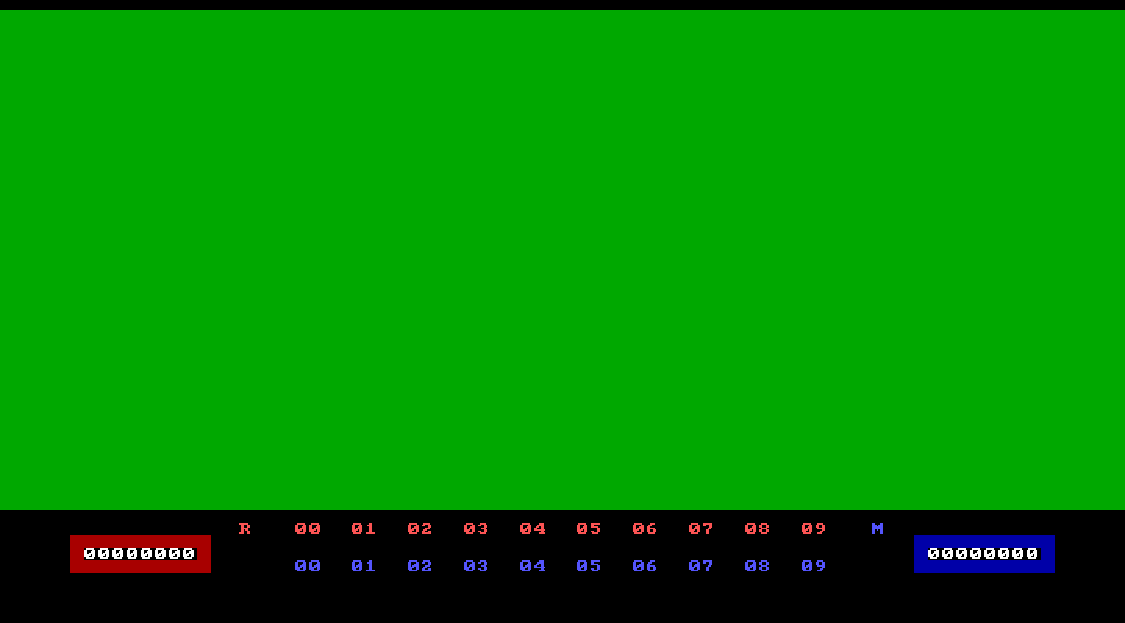
\includegraphics[scale=0.6]{img/Pantalla.pdf}
	\caption{Pantalla inicial.}
\end{figure}


\subsection{Ejercicio 2}
\justify
Inicialmente modificamos los archivos \textit{idt.c} e \textit{idt.h} para completar las entradas de la IDT. Definimos a la IDT como un arreglo de idt_entry_t de 255 posiciones, que primero inicializamos en cero, y el descriptor de la IDT (IDT_DESC), indicando el tamaño y la dirección de la IDT. Para inicializar las entradas de la IDT utilizamos un \textit{DEFINE} que, dado el número de la interrupción, completa los campos del descriptor de la IDT correspondiente. Para el caso de las interrupciones de software el DPL es 3, dado que las mismas deben poder ser accedidas por las tareas y en los demás casos el DPL es 0, ya que no deben poder ser accedidas por las tareas. En todos los casos el selector de segmento es de código de nivel 0, porque las rutinas no pueden ser modificadas por las tareas. Como la dirección de la IDT no está definida en tiempos de compilación fue necesario definir una función llamada idt_init que inicializara las entradas de la IDT en tiempos de ejecución. Definimos 21 entradas en la IDT para las excepciones del procesador(de 0 a 20).
\justify
Para imprimir las excepciones en la esquina superior izquierda de la pantalla  cuando estas ocurren, implementamos la función "print_exception", que se encuentra en el archivo \textit{screen.c}. La misma es llamada inicialmente en el código de \textit{isr.asm}, aunque luego esto será modificado como se ve en el código, ya que esta acción será realizada por el modo debug. 


%Acá va una imagen de un descriptor de la IDT.


\subsection{Ejercicio 3}
\justify
En este ejercicio definimos dos entradas en la IDT para las interrupciones externas o de hardware (32 del clock y 33 del keyboard) y cuatro entradas para las interrupciones de software(88, 89, 100, 123).
\justify
De acuerdo a lo pedido en el segundo, tercer y cuarto item, dentro del archivo \textit{isr.asm} escribimos el esqueleto de las rutinas de interrupciones del reloj, de teclado y de software, que luego irán siendo modificadas a lo largo del transcurso de los ejercicios.

\justify
\textbf{Rutina de interrupción del reloj}
\justify
Esta rutina comienza con un call a la función pic_finish1, para avisar que la interrupción fue atendida. Seguidamente se llama a la función "next_clock", provista por la cátedra. La misma se encarga de imprimir por pantalla una animación del un cursor rotando en la esquina inferior derecha de la pantalla.

\justify
\textbf{Rutina de interrupción del teclado}
\justify
Esta rutina comienza levantando del puerto 0x60 la tecla que fue presionada durante la interrupción. Para que esta tecla sea impresa por pantalla se implementó la función "print_digito" \ en el archivo \textit{screen.c}. Para finalizar, hacemos un call a pic_finish1, para avisar que la interrupción fue atendida.

\justify
\textbf{Rutinas de interrupciones de software}
\justify
Las rutinas de interrupciones de software solo mueven a eax los números indicados por el item d, esto luego será modificado.

\subsection{Ejercicio 4}
\justify
Para inicializar el directorio y las tablas de páginas del kernel, implementamos la función ``mmu_init_kernel_dir", que crea un directorio y una tabla de páginas (tabla_0) del tipo \textit{page_directory_entry}  y \textit{page_table_entry}, respectivamente. Estas estructuras fueron definidas en el archivo \textit{mmu.h} y siguen el formato de las entradas al directorio y a la tabla de páginas. Una vez creados los inicializamos en 0.
\justify
La primera entrada del directorio (directorio[0]) va a mapear a la tabla de páginas creada y esta mapeará a todo el kernel, por lo que completamos el campo de la base del directorio[0] con la dirección de la tabla de páginas. El privilegio de esta entrada es 0. Una vez mapeado el directorio a la primera tabla de páginas, mapeamos la misma al kernel, usando identity mapping. Nuevamente, el privilegio de cada entrada de la tabla de páginas es 0. Al final de la rutina devolvemos la dirección del directorio de tablas de páginas. 
 
\justify  
Ya creadas las funciones para inicializar el directorio y la tabla de páginas, escribimos en \textit{kernel.asm} el código necesario para activar paginación: inicializamos el manejador de memoria y el directorio de páginas mediante un call a la función ``mmu.init" \ y ``mmu_init_kernel_dir", respectivamente. Luego, cargamos en el registro cr3 la dirección del directorio y activamos paginación seteando en 1 el bit 31 de cr0.

\begin{figure}[h]
	\centering
	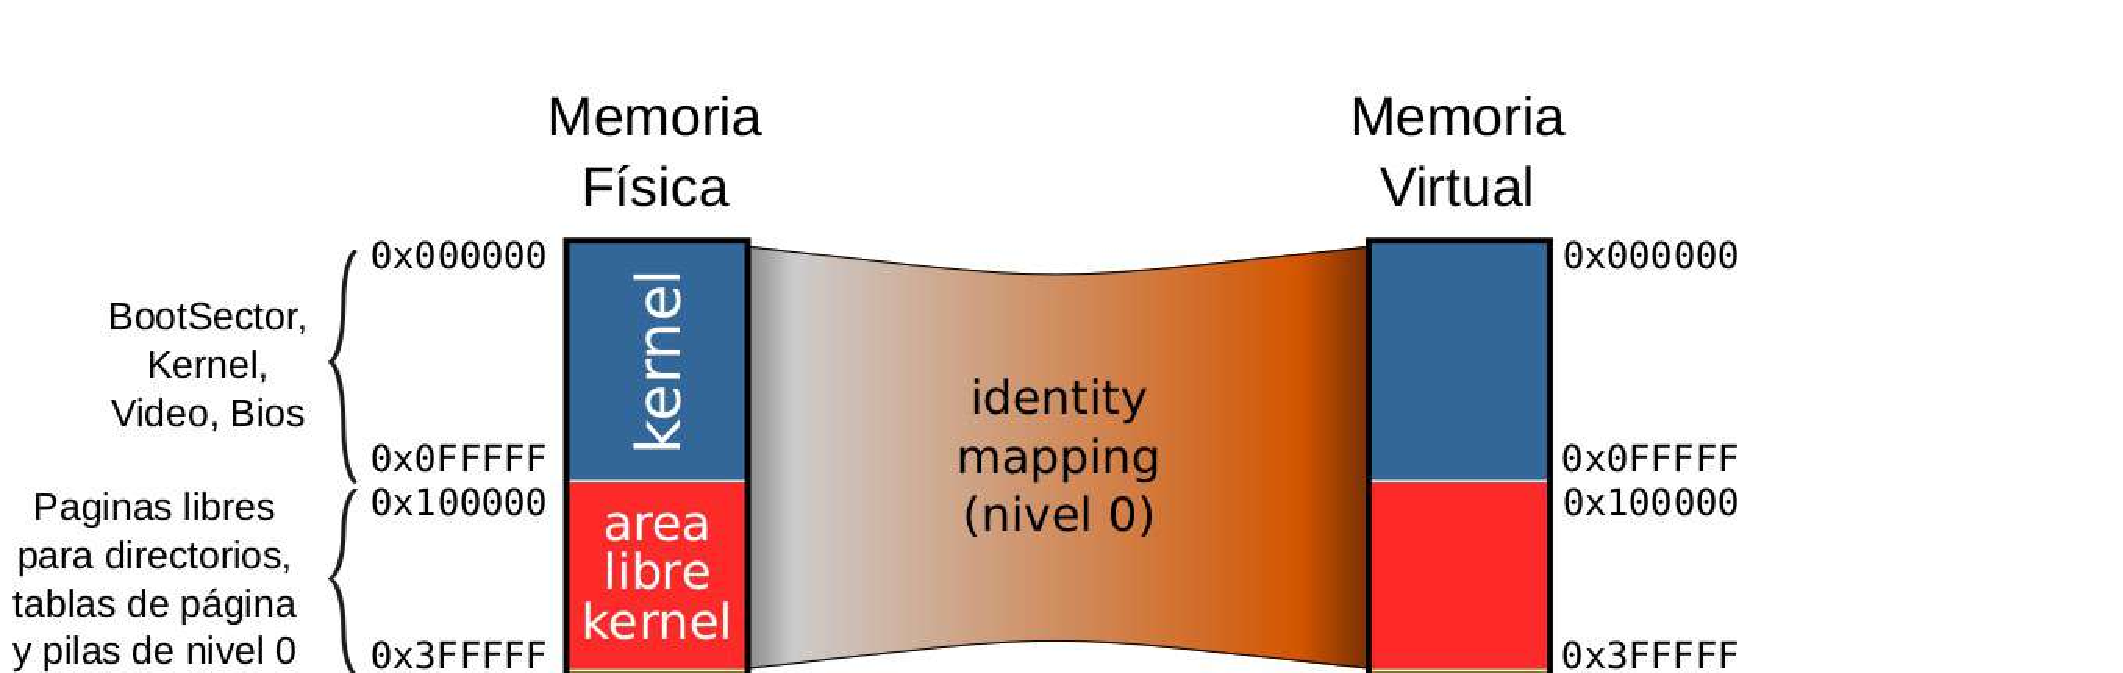
\includegraphics[scale=0.5]{img/MapearKernel.pdf}
	\caption{Mapeo del kernel.}
\end{figure}

\newpage
\subsection{Ejercicio 5}
\justify
Inicialmente y siguiendo lo indicado por el primer item, completamos la función ``mmu_init" \ con la dirección de la primera página libre del kernel (0x100000), y luego completamos la función ``mmu_next_free_kernel_page" \ para que nos devuelva la dirección de la próxima página libre del área libre del kernel.
\justify
Implementamos la función ``mmu_map_page" que, dado un cr3, una dirección virtual, una dirección fisica y unos atributos, mapea ambas direcciones. Lo primero que realiza esta función es obtener de la dirección virtual el índice del directorio de tabla de páginas y el índice dentro de la tabla de páginas. Luego se fija si la tabla de páginas de esa page_directory_entry está presente y, en caso de que no, la crea pidiendo la próxima página libre del área del kernel y la inicializa con todas las entradas en 0. Una vez creada la tabla de páginas, se completa la entrada correspondiente de la page_directory_entry con la base de la tabla de páginas, los atributos pasados por parámetro.

\justify

 



\subsection{Ejercicio 6}
\subsection{Ejercicio 7}
\subsection{Ejercicio 8}



\end{document}

